\chapter{Evaluace}

V rámci této kapitoly se zaměříme na otestovaní konverzního mechanismu platformy nad daty nastiňující reálnou situaci na úřadech.

V únoru roku 2015 vydalo Ministerstvo vnitra dopadovou studii na odhad nákladů k zavedení zákona o registru smluv\footnote{http://www.janfarsky.cz/wp-content/uploads/2015/05/Dopadov\%C3\%A1-studie-ke-KPN-k-registru-smluv-PRACOVNI-VERZE-27-02-2015-1.pdf}. V reakci na tento odhad nedlouho poté vydalo Cetrum aplikované ekonomie o.s. stínový výpočet korigující výsledky Ministerstva vnitra\footnote{ http://www.rekonstrukcestatu.cz/publikace/2015-03-04-stinovy-vypocet-ria-k-registru-smluv.pdf}. Na základě těchto studií můžeme získat hrubou představu o tom, kolik jednotlivé subjekty cca uzavírají nedlouho poté smluv. Veřejné instituce tak rozdělíme do čtyř kategorií:  

\begin{itemize}
\item Malé - Nejmenší instituce, uzavírající jednotky smluv měsíčně s celkovým úhrnem maximálně několika desítek smluv ročně (v rámci měst a obcí jde o nejvyšší zastoupení).
\item Střední - Subjekty generující maximálně desítky smluv měsíčně, s jednotkami stovek smluv ročně (v rámci všech subjektů pravděpodobně nevýznamnější zastoupení). 
\item Středně velké - Instituce, které produkují desítky, až stovky smluv měsíčně s jednotkami tisíců smluv ročně.
\item Velké - Velké instituce se stovkami až tisíci smluv měsíčně s roční produkcí tisíců až desetitisíců smluv.
\end{itemize}

Pro simulaci prostředí jednotlivých kategorií vytvoříme pro každou skupinu testovací relační databázi s desítkami, stovkami, tisíci a desetitisíci smluv. Nad každou databází spustíme konverzní modul a změříme dva pravděpodobně nejčastější požadavky - dump dat, resp. výčet všech smluv a vyhledání jedné konkrétní smlouvy. Dump je základní funkcionalitou k vypublikování otevřených smluv. Potřebujeme ho také v rámci platformy, resp. jednotného úložiště, které dílčí dumpy stahuje. Ukázka vyhledání jedné smlouvy slouží spíše k ukázce, že konverzní modul půjde využít i mimo platformu, např. v rámci webových stránek konkrétní veřejné instituce.   

Pro generování dat v SQL databázi byl zvolen nástroj Sql Data Generator\footnote{TODO - odkaz na zdroj.}. Tento nástroj umožňuje nastavení nejen počtu vygenerovaných dat, ale i např. procentuální zastoupení propojení tabulek nebo šablony pro konkrétní hodnoty v jednotlivých sloupcích. Umožní nám přiblížit se k reálnému obsahu databází veřejných institucí\footnote{Pro představu je příklad XML scriptu přiložen na datovém nosiči. Sql Data Generator je ale komerční nástroj, který neumožňuje zobrazit generovaný sql příkaz.}. K samotnému profilingu využijeme klasických prostředků prostředí .Net. Změříme dobu od přijmutí požadavku po jeho kompletní zpracování.
\newpage

Měření probíhalo na sestavě:
\begin{itemize}
\item Intel Core i5-4200U, CPU @ 1.60GHz - 2.30GHz
\item 4GB RAM
\item 64bit operační systém
\item Databáze - MS SQL 2014
\end{itemize}

Pro každou kategorii bylo provedeno 15 měření pro dump, resp. vyhledání smlouvy. Z každé sady výsledků se odebrala minimální a maximální hodnota a následně ze zbývajících hodnot byl vypočítán průměr. Pro názornost, u dumpu uvádíme také velikost výstupních dat a počet vygenerovaných trojic. Výsledky lze najít v následujících grafech (\ref{obr:graphDump1},\ref{obr:graphDump2},\ref{obr:graphGet1}).

\begin{figure}[H]
\centerline{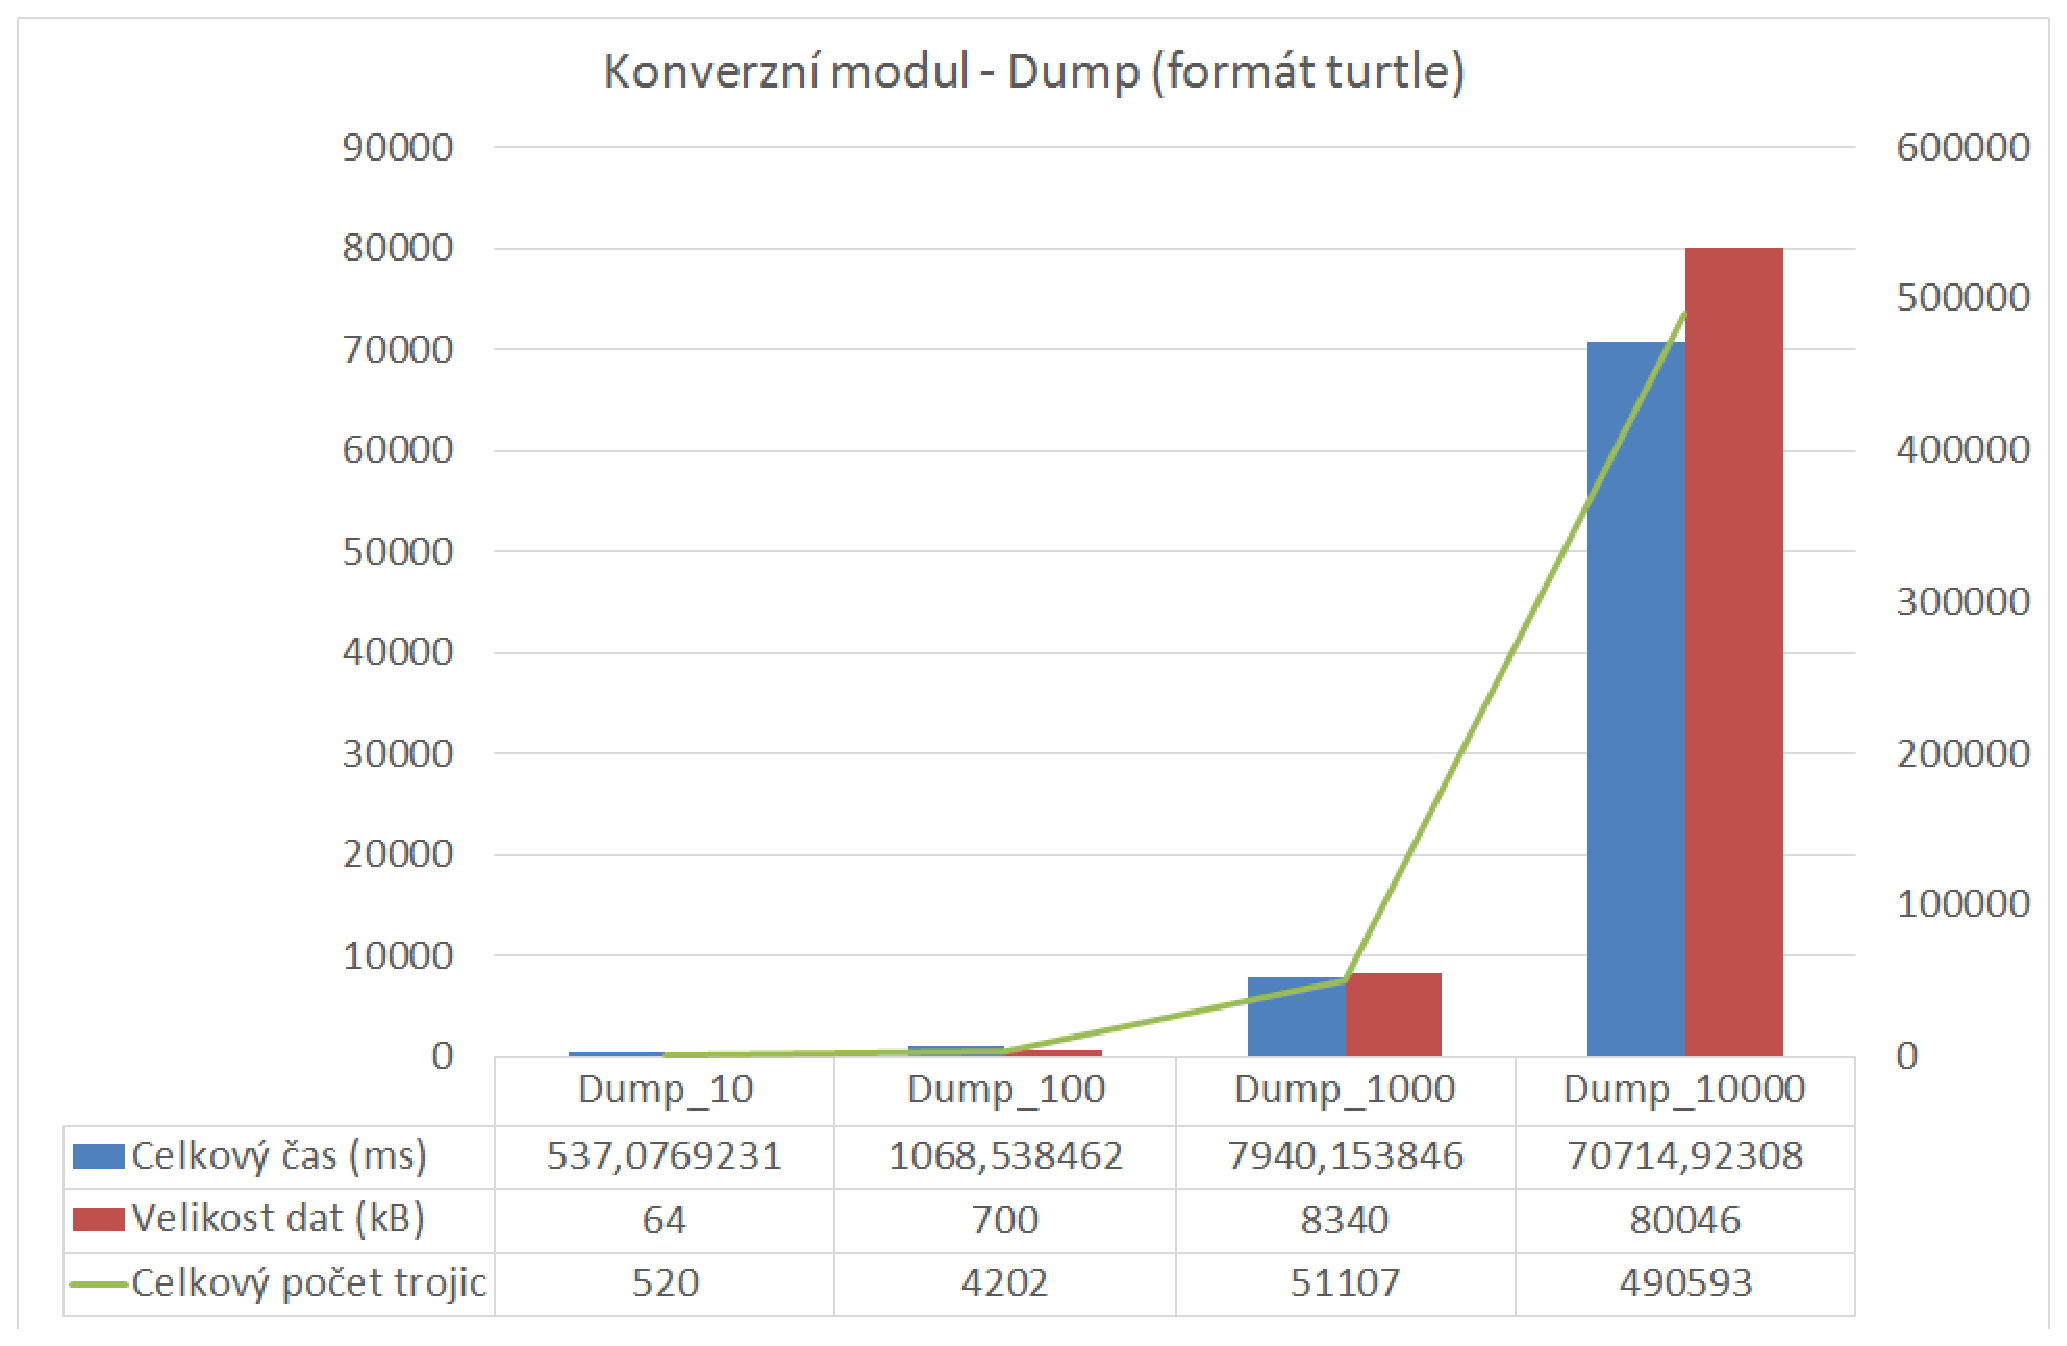
\includegraphics[width=\textwidth]{img/graphDump1.eps}}
\caption{Znázornění časové náročnosti dumpu vybraných dat}
\label{obr:graphDump1}
\end{figure}

\begin{figure}[H]
\centerline{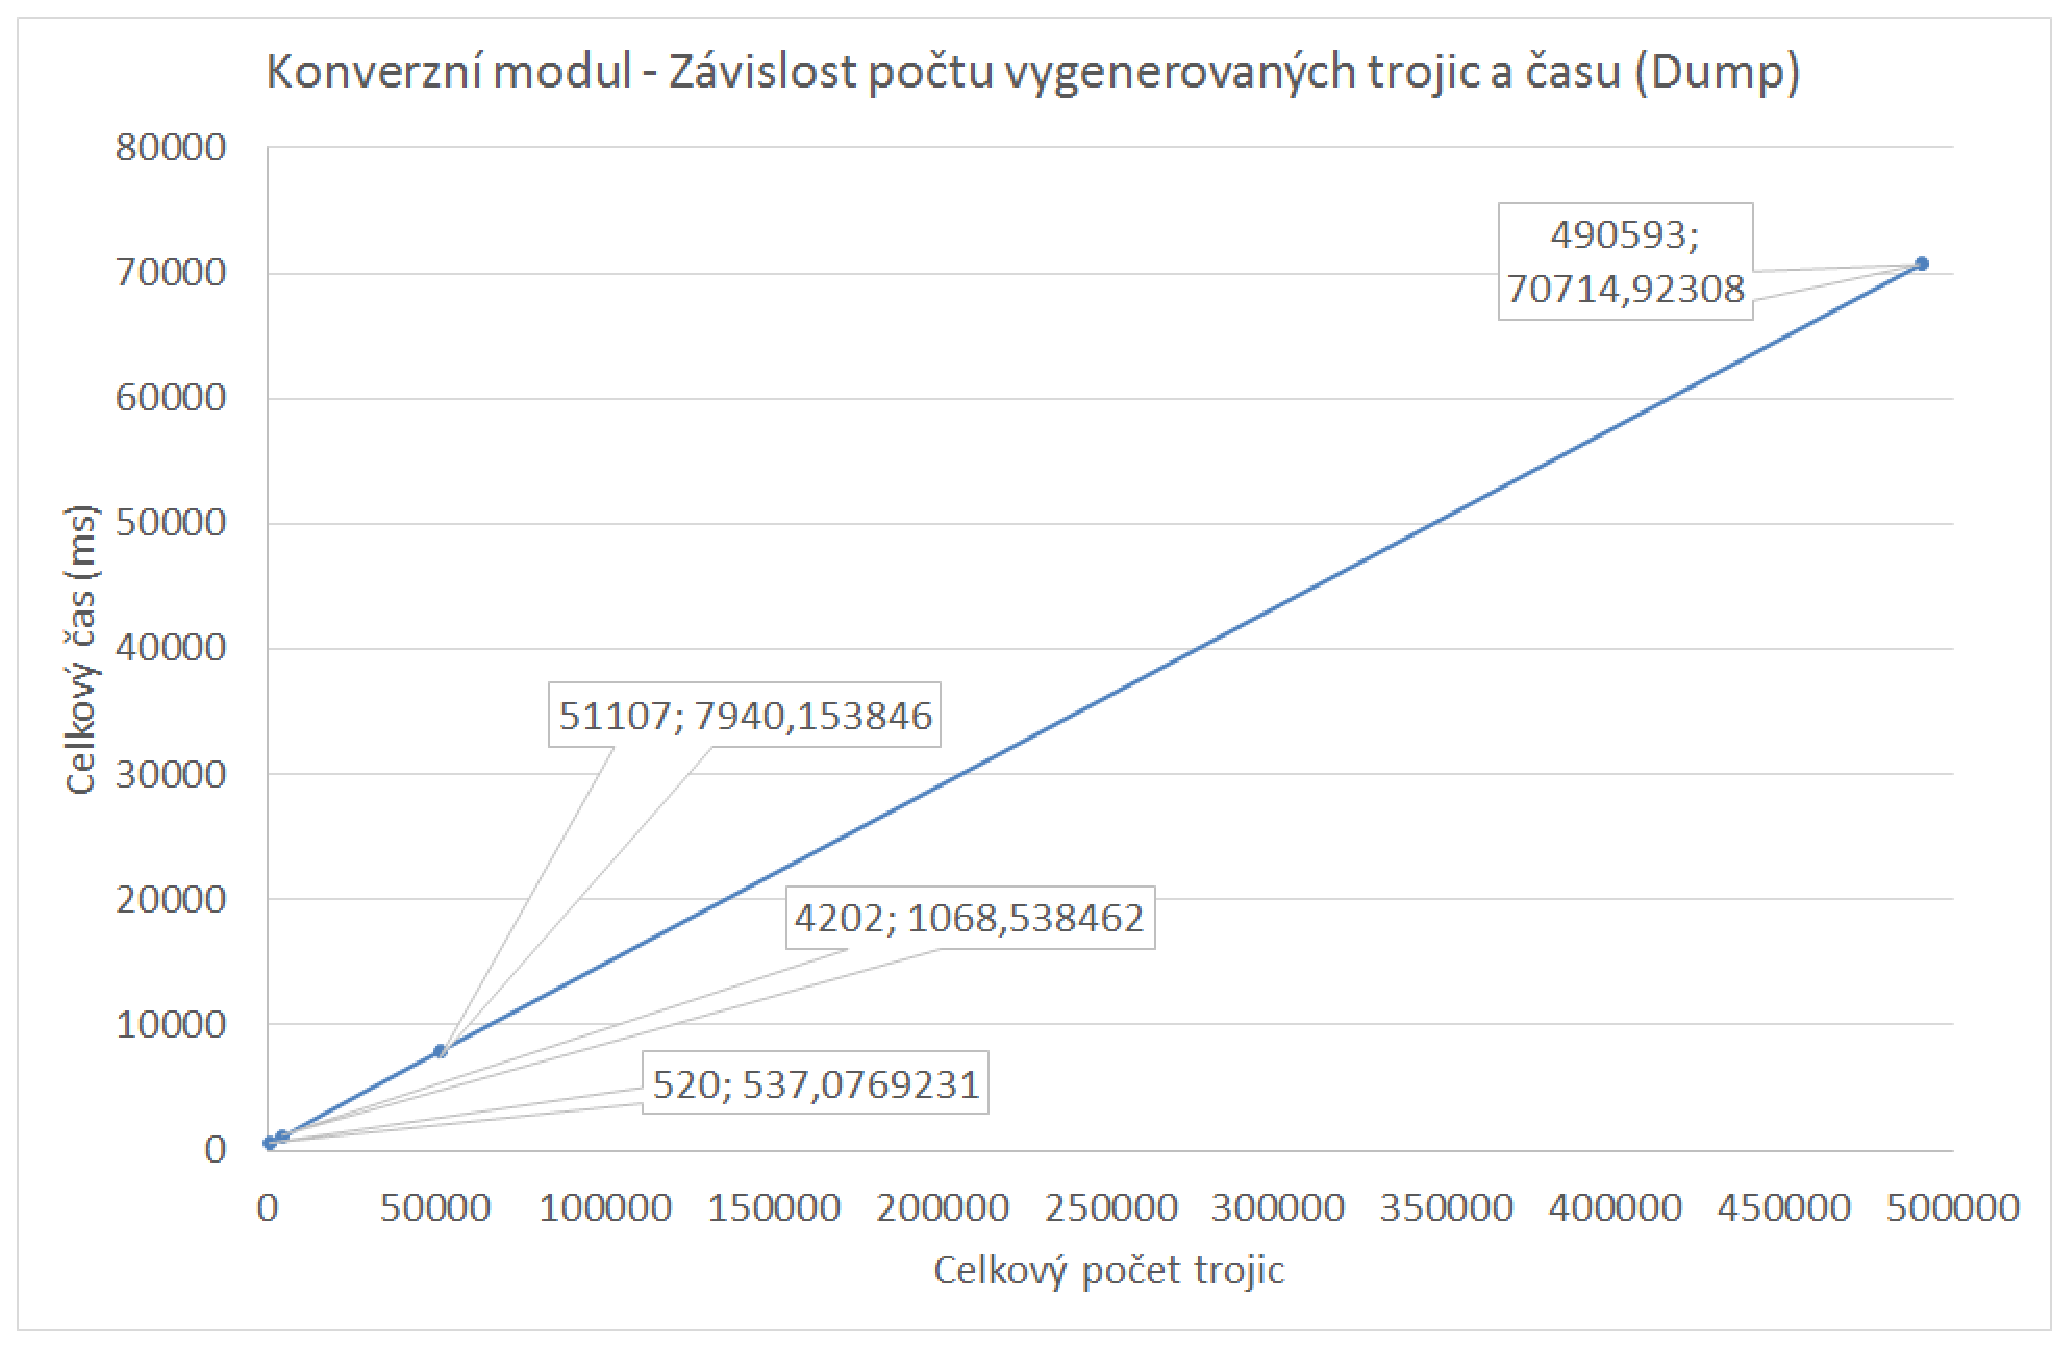
\includegraphics[width=\textwidth]{img/graphDump2.eps}}
\caption{Znázornění vztahu počtu vygenerovaných trojic a času při dumpu vybraných dat}
\label{obr:graphDump2}
\end{figure}

\begin{figure}[H]
\centerline{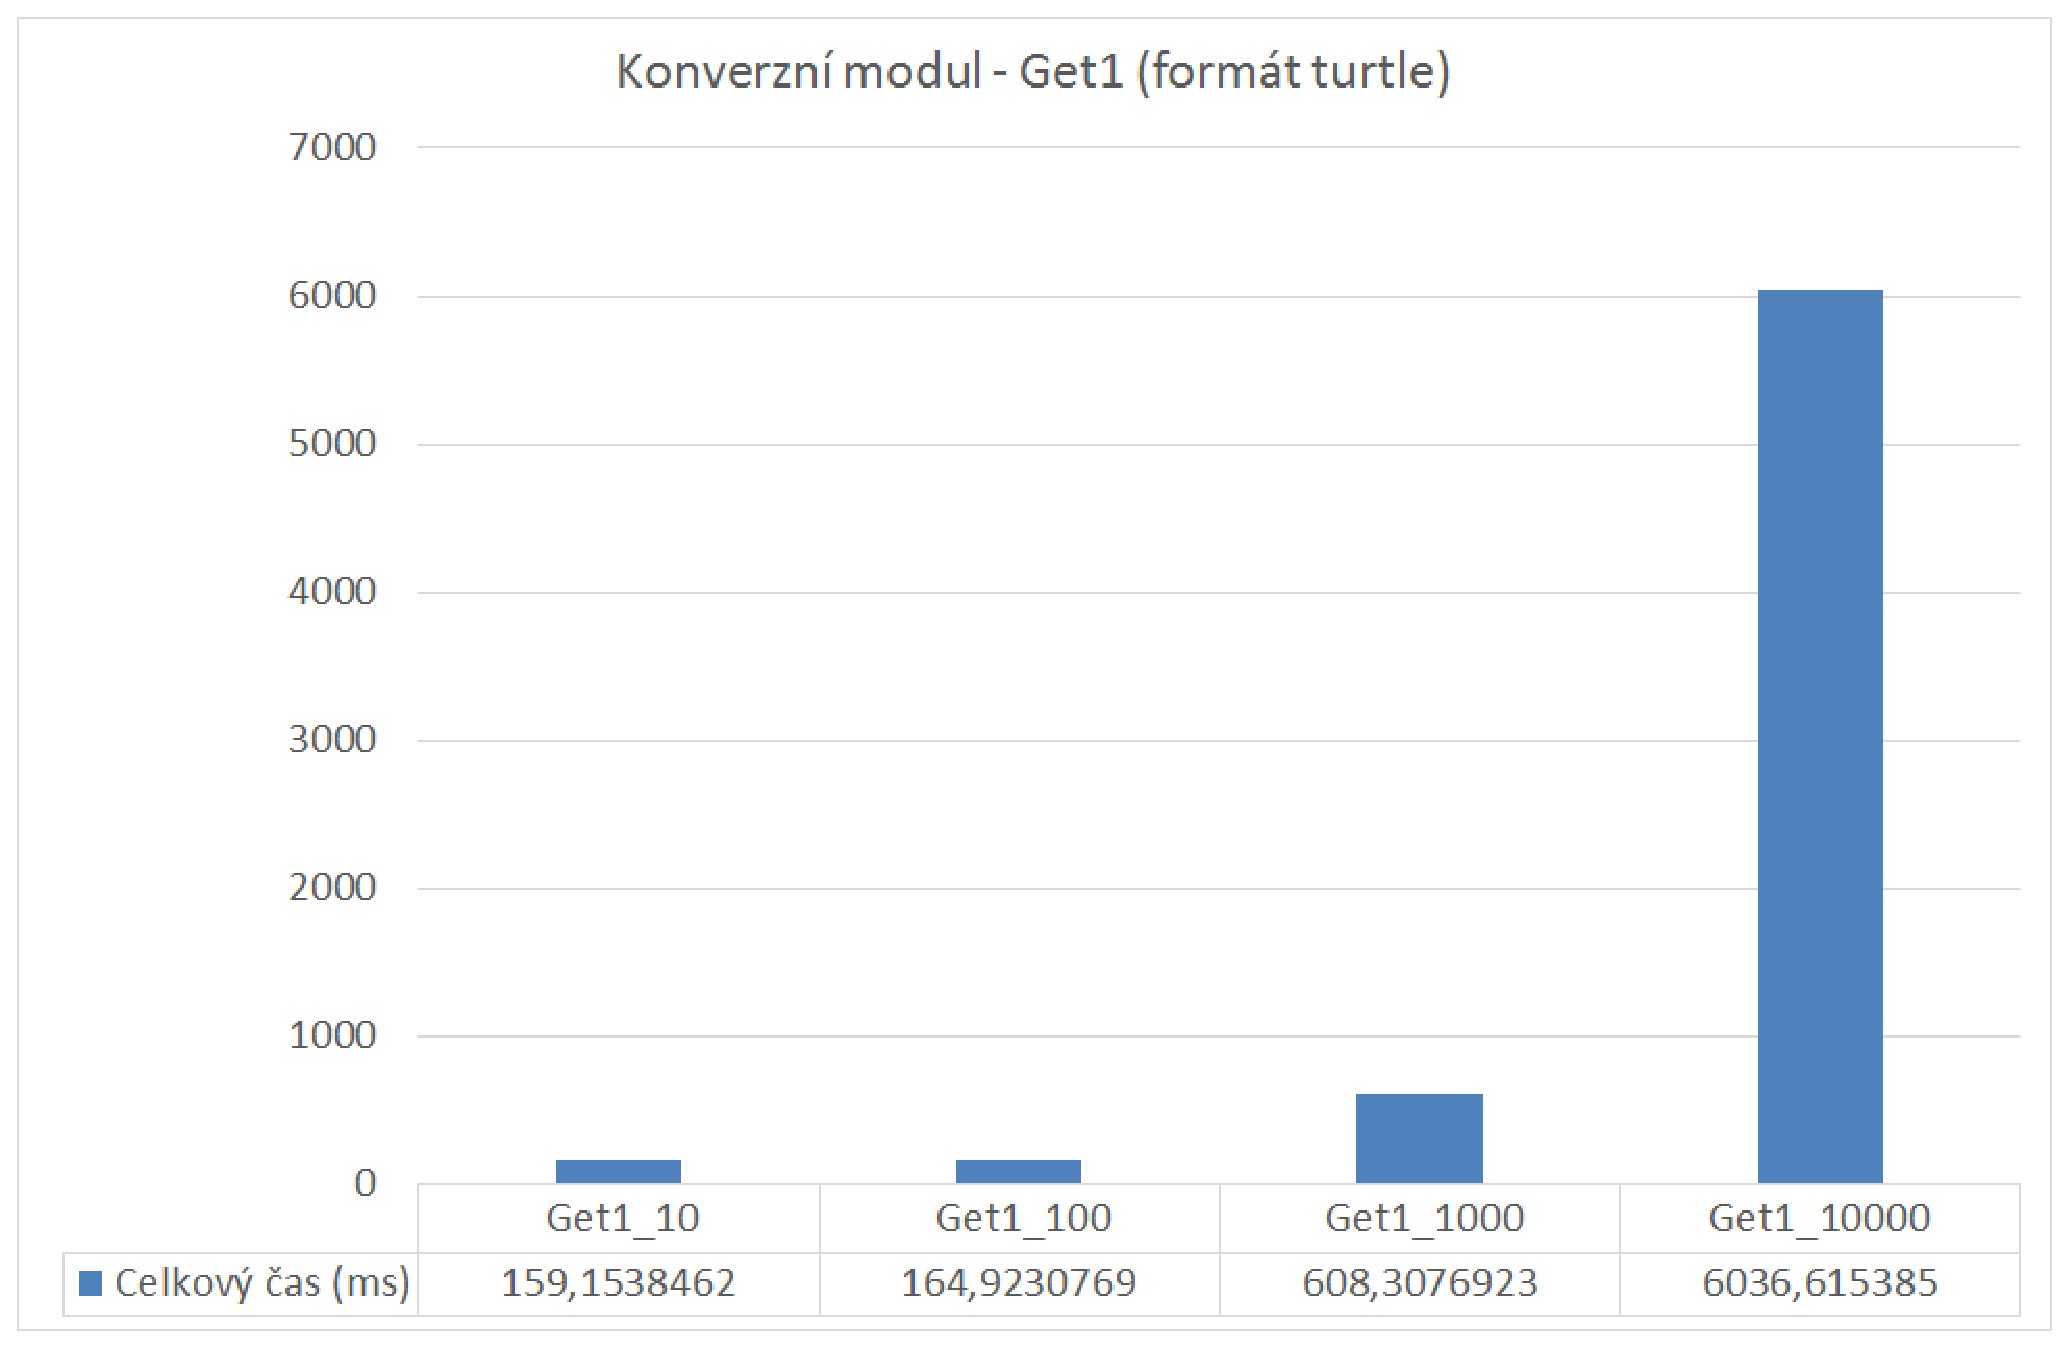
\includegraphics[width=\textwidth]{img/graphGet1.eps}}
\caption{Znázornění časové náročnosti získání jedné smlouvy u vybraných dat}
\label{obr:graphGet1}
\end{figure}

\newpage
Z výsledků lze konstatovat, že výkon klesá cca lineárně s množstvím dat (viz. graf \ref{obr:graphDump2}). Můžeme říci, že konverzní modul je schopen poskytovat základní funkcionalitu v rozumném čase u menších, středních i středně velkých institucí. U velkých institucí už výsledky nejsou ideální. Institucí publikujících takové množství smluv je ale v prostředí České republiky velmi málo. Příslibem je také to, že využívaný R2RML procesor podléhá soustavnému vývoji a do budoucna lze očekávat výrazné zrychlení.
